\documentclass[preprint,12pt]{elsarticle}%

%% Use the option review to obtain double line spacing
%% \documentclass[authoryear,preprint,review,12pt]{elsarticle}

%% Use the options 1p,twocolumn; 3p; 3p,twocolumn; 5p; or 5p,twocolumn
%% for a journal layout:
%% \documentclass[final,1p,times]{elsarticle}
%% \documentclass[final,1p,times,twocolumn]{elsarticle}
%% \documentclass[final,3p,times]{elsarticle}
%% \documentclass[final,3p,times,twocolumn]{elsarticle}
%% \documentclass[final,5p,times]{elsarticle}
%% \documentclass[final,5p,times,twocolumn]{elsarticle}

%% \usepackage{amssymb}
%% \usepackage{amsthm}

\journal{Computers In Human Behavior}%

%%%%%%%%%%%%%%%%%%%%%%%%%%%%%%%%%%%%%%%%%%%%%%
\usepackage[utf8]{inputenc}%                 %
\usepackage[T1]{fontenc}%                    %
\usepackage[hidelinks]{hyperref}%            %
\usepackage{subcaption}%                     %
\graphicspath{{../github/img/}}%       %
%                                            %
\usepackage{xcolor}%                         %
\newcommand{\gnramos}[1]{\textcolor{red}{#1}}%
%%%%%%%%%%%%%%%%%%%%%%%%%%%%%%%%%%%%%%%%%%%%%%

\begin{document}

\begin{frontmatter}

%% Title, authors and addresses

%% use the tnoteref command within \title for footnotes;
%% use the tnotetext command for theassociated footnote;
%% use the fnref command within \author or \address for footnotes;
%% use the fntext command for theassociated footnote;
%% use the corref command within \author for corresponding author footnotes;
%% use the cortext command for theassociated footnote;
%% use the ead command for the email address,
%% and the form \ead[url] for the home page:
%% \title{Title\tnoteref{label1}}
%% \tnotetext[label1]{}
%% \author{Name\corref{cor1}\fnref{label2}}
%% \ead{email address}
%% \ead[url]{home page}
%% \fntext[label2]{}
%% \cortext[cor1]{}
%% \address{Address\fnref{label3}}
%% \fntext[label3]{}

\title{Brazilian School Girls' Perspectives on a Computer Science Major: Mining Association Rules}

\author{Maristela Terto de Holanda\corref{cor1}\fnref{label1}}%
\ead{mholanda@unb.br}%
\ead[url]{http://cic.unb.br}%
\author{Roberto Mourão}%
\author{Aleteia Araújo}%
\author{Maria Emília Walter}%
\author{Guilherme N. Ramos}%


%% use optional labels to link authors explicitly to addresses:
%% \author[label1,label2]{}
%% \address[label1]{}
%% \address[label2]{}

\address{Department of Computer Science, University of Brasília, Brasília, Brazil}%

\begin{abstract}
The field of Computer Science (CS) has been of little interest for girls straight out of high school, when considering undergraduate majors in Brazil. At the University of Brasília’s CS Department, female students compose less than 10\% of the student body. In an effort to understand the girls’ lack of interest in computer related courses, we applied an anonymous questionnaire, from 2011 to 2014, regarding their perceptions of the field.  The participants were 3707 females students who completed an anonymous questionnaire. We applied Association Rules in Data Mining to analyze the responses discovering that the family's approval of such choice is one of the most important factors. The knowledge gained through this study could guide future research on the matter and guidelines for motivating girls to pursue careers in Computer Science.
\end{abstract}

\begin{keyword}
%% keywords here, in the form: keyword \sep keyword
computer science \sep gender \sep girls \sep women \sep female student \sep data mining \sep association rules \sep apriori%

%% PACS codes here, in the form: \PACS code \sep code

%% MSC codes here, in the form: \MSC code \sep code
%% or \MSC[2008] code \sep code (2000 is the default)
\end{keyword}

\end{frontmatter}

%% \linenumbers

%% main text
\section{Introduction}\label{sec:intro}%

%Begin Maristela
In Brazil, the choice of an undergraduate major in the area of Computer Sciences is not among the top choices for girls in high school when contemplating a career. As \cite{maia_2016} presents, between 2000 and 2013 in Brazil, an average of only 17\% of all graduates in various Computer Science majors were women. This research covered majors in Computer Science, Computer Engineering, and Information Systems, among others. Particularly, in the Federal District, at the University of Brasilia, which currently has approximately 30,000 students enrolled in undergraduate programs, the reality is even worse, where in the past 10 years, according to \cite{couto_2014} only 10\% were women.

	Responding to the low incidence of women in Computer Science majors, recently researchers have given much thought about how to improve this scenario and proposed strategies to encourage girls to pursue a profession in the Computer Sciences   \cite{cohoon_2002} \cite{couto_2014}  \cite{gurer_2002}  \cite{maia_2016}. Brazil and other countries have developed initiatives to debate this issue. Specifically, the Institute of Electrical and Electronics Engineers (IEEE) has a program which address the problem: the IEEE Women in Engineering (WIE) \cite{wie2017}. The WIE is a major professional and international organization dedicated to promoting women scientists and engineers. Another prominent program in promoting women in the area of Computers is ?Girls who Code? \cite{girlsWC_2017}, which has over 40,000 members and various initiatives to increase the participation of girls in Computer Sciences over various regions in the United States. Another initiative from the United States is the ?Grace Hopper Celebration of Women in Computer Sciences? event, which is the biggest event worldwide for discussing the theme of women in the field. In 2016 alone 15,000 people from 87 countries participated in the 700 presentations \cite{GHC_2017}.

	In Brazil, since 2007, the Brazilian Society of Computing Conference held the Women in Information and Technology Workshop (WIT), to discuss the theme. Brazilian governmental agencies, such as the Ministry of Science and Technology released calls for submissions of research projects specifically related to the education of girls in Computing or Physical Science majors \cite{cnpq_2017}. Aiming to gather information about the perceptions of high school girls regarding computer science, the Department of Computer Science at the University of Brasilia, developed the project, Meninas.comp: computação  tambem e coisa de menina, Girls.comp: computer science is a girl thing too.

%End Maristela

\gnramos{Falar da análise realizada (Roberto e Guilherme)}%

Between the years of 2012 and 2014, we contacted thousands of girls in Middle and High School to investigate the relationship between their intention to apply for an undergraduate course in Computer Science and their affinity with the field and computing tools. We used the Apriori algorithm on the collected data, searching for interesting association rules and insights on the girls' interest in CS and their background.

This following sections of this work are organized as follows: Section~\ref{sec:background} presents related work and background information on this approach, Section~\ref{sec:mining} describes details of the data mining applied, Section~\ref{sec:results} provides our experimental results and our finds and Section~\ref{sec:conclusion} presents concluding remarks.
%
\section{Related Works}\label{sec:related}%
There have been several studies addressing the gender issue in Computer Science. Lagesen describes CS as STEM field that has excluded women~\cite{vivian_2007}. Putnik et al. presents data from Yugoslavia, comparing gender ratios and observing a higher number of men compared women~\cite{zoran_2017}.

Stout et al. in~\cite{jane_2016} and Cheryan et al. in~\cite{sappa_2013} provide studies about stereotyping in Computer majors, also arguing that there is a higher ratio of men than women in this field in the US. Likewise, Mercier et al. present surveys, drawings, and interviews which were used to examine the perception of US middle school students about characteristics of knowledgeable computer users~\cite{Mercier_2006}. These results showed cultural stereotypes of a computer user: 89\% were male and 94\% wore glasses.

Keinan et al. show data that the ratio of graduated women from Bachelor's programs in CS was of almost 40\% in 1984, dwindling to 20\% by 2006 in the US~\cite{keinan_2017}. Vardi has similar results, and adds that in 2013 and 2014, only 14.7\% of those graduates were women~\cite{moshe_2015}.

Papastergiou used descriptive statistics, principal component analysis and analysis of variance in~\cite{papastergiou_are_2008} to investigate 358 Greek high school students' intentions and motivation for pursuing academic studies in CS. This study looked into several factors, such as the influence of family and academic environment on their career choices, their perception of a professional career in CS, and their self-efficacy beliefs regarding computers. The analysis showed that a lack of exposure to and use of a computer at home and in school from early stages in the students' lives seems to be the main factor in discouraging them from studying CS, specially considering the data for girls.

Anderson et al. applied means, \mbox{Mann-Whitney} $U$ test comparison, and non-parametric statistics in~\cite{anderson_because_2008} to study possible factors related to low rates of female participation in education pathways leading to information and communications technology (ICT) professions, considering data from a three-year period. The survey had binary options, such as ``I am very interested in computers'' and ``I am not interested in computers'', was presented to 1,453 high school girls in their Senior year. The study identified two factors associated with a woman's aversion to ICT careers: the perception that the subject is boring, and an intense dislike of computers.

Maia describes a similar situation in~\cite{maia_2016}, presenting a study on female participation in university majors in CS in Brazil, based on the Higher Education Census data from the Ministry of Culture and Education between the years of 2000 and 2013. One of the issues raised was that while the number of male graduates increased 98\% in the period, that of female graduates decreased 8\%.

The Department of Computer Science\footnote{\url{http://cic.unb.br}} at the University of Brasília (UnB) currently offers three undergraduate degrees related to CS: Bachelor of Computer Science (since 1987), Licentiate in Computing (since 1997), and Computer Engineer (since 2008). Figure~\ref{fig:computerMajorUnB} shows gender data for students enrolled in them.

\begin{figure}%
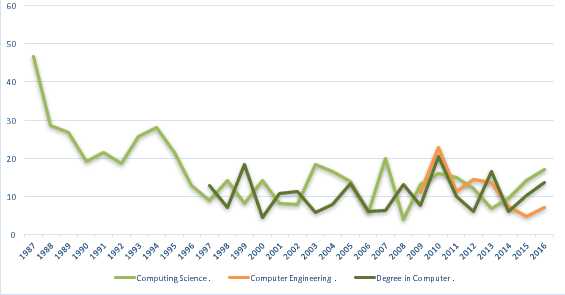
\includegraphics[width=\textwidth]{img/Figure1-girlsUnB}%
\caption{Ratio of female students enrolled in UnB's CS majors.}%
\label{fig:computerMajorUnB}%
\end{figure}%

In 1987, when the Bachelor course began, the gender difference between students enrolled was relatively low: 47\% of were female. However, this number decreased over time and, in 1997, this percentage fell to 10\%; by 2013 it was only 6\%. The Licentiate degree's ratio oscillates roughly around 11\%, while the Computer Engineer, which already began with low numbers, saw them fall to less than 12\% in the past three years.

We can see from the data that the difference between the number of male and female students enrolled in a CS major at UnB has decreased over the years, similar to what was reported in the before mentioned surveys. Given this alarming decline, and the widening disparity between male and female representations in the field of Computer Science, our work aims to investigate possible reasons for such scenario.\gnramos{Acho que poderia ficar explícito o porque da necessidade de mais mulheres. (``o que a diversidade acrescenta?'' e o que poderia ser feito com os resultados para melhorar a situação)}
%
\section{Data Collection and Analysis}\label{sec:data}
The enrollment of female students in Computer Science majors is decreasing every year and one of the biggest challenges in addressing this is to discover what motivates girls to avoid a CS major. Some issues have been outlined in the literature, such the impact of associated stereotypes; but our research intends to further investigate the women's perceptions of the Computer Science field by looking at the prospective enrollees: girls in high school. There is a significant lack of research on this subject in Brazil, and we believe such analysis could aid in the proposal of policies for increasing female participation in the field.

\subsection{Survey}
The members of the \texttt{Meninas.comp} from the University of Brasilia developed a questionnaire to inquire about female high school students' perceptions of the Computer Science field. It included personal profile questions, such as sex, school year, field of interest for a college education, interest in a career in CS, and others; as well as more general questions related to computers, such as: where the student uses computers and for what kind of tasks.

From 2011 to 2014, the questionnaires were given to female high school students in the Federal District, during during Brazil's Ministry of Science and Technology's National Science and Technology Week\footnote{\url{http://semanact.mcti.gov.br/}} activities.

% Finally, the questionnaire comprised specific (yes, no, maybe) questions regarding the prestige of working with computers and wages earned working with computers, among others:
% Does a university computer science course only teach how to use software?;
% Does a university computer science course require few math skills?;
% Are the majority of Computer Science majors male?;
% Is it necessary to know how to use a computer to enroll in a university computer course?;
% Is it necessary to work in computer sciences to enroll in a computer course?;
% Would your family like you to take the college entrance exam for Computer Sciences?;
% Is it difficult to find work in computer sciences after graduating?;
% Do people who work in computer sciences have little leisure time?;
% Does working in computer sciences allow you to exercise your creativity?;
% Is working in computer sciences prestigious?; and
% Does working in computer sciences pay well?.


% \subsubsection{Research Data}%

There were 1,821 responses in 2011, 944 in 2012, 517 in 2013, and 425 in 2014; adding up to a total of 3,707 completed questionnaires. The decrease of respondents in the period is due to the project's context, the amount of work possible is directly affected by the number of volunteers working on it. In 2011, there were 5 Professors and 10 students members, but they dwindles to only 1 Professor and 5 students (working few hours) in 2014. The collected data was consolidated in a spreadsheet and analyzed.

% Subsequently, in the data preparation phase, we received the collection data in 4 spreadsheets, one by year. Then, the columns of the spreadsheets were reorganized. This reorganization was applied to the 4 spreadsheets, corresponding to 2011, 2012, 2013, and 2014. The organization of the answers were tabulated and served as the source for the creation of a single table, comprising 35 attributes. The main attributes used in the analysis of this paper were: Bring\_Prestige, Computer\_Friends, Computer\_Lan\_House, Computer\_Relatives , CS\_Interest, Family\_Approval, Good\_Salary, Low\_Leisure, Use\_Creativity, Computer\_Home, Computer\_Library, Computer\_School,  CS\_Choice, Educational\_Stage, Field\_Interest, Has\_Low\_Math, Low\_Employability, Man\_Majority and Year.

% Finally, the data were filtered so that of the 3,707 questionnaires,  researchers excluded those answered by students who: were already in higher education;  were male;  failed to answer the key question: \textit{Are you interested in doing a major in Computer Sciences?}. This left 3,161 questionnaires to be analyzed.


\subsection{Data Analysis}\label{sec:analysis:related}%

Data analysis includes, among other things, procedures for analyzing data and techniques for interpreting their results~\cite{Tukey1962}, while Data Mining is the process of discovering insightful patterns and predictive models from data~\cite{Zaki2014}, in an effort to make sense of usually large amounts of information in some domain~\cite{Cios2007}. Our primary focus is the gender gap in pSTEM careers, so our study aims to characterize the profiles of girls who intend to enroll in undergraduate studies, especially those interested in Computer Science.

One of the possible approaches to finding interesting relationships in data is \emph{association rules mining}~\cite{Cios2007}, which produces easily understandable results as rules states as ``\emph{if A occurred, then B occurs}''. For example, it is likely that a rule ``\emph{if a girls sees the CS field as boring, she will not enroll in a CS major}'' is found. This processing may require a lot of resources, and a computationally feasible solution is the \emph{Apriori} algorithm, which uses only the itemsets found large in the previous pass to generate candidate itemsets~\cite{Agrawal1994}, and produces the rules with the highest \emph{confidence} (how often the rule has been found to be true), despite their \emph{support} (number of occurrences)~\cite{taniar_exception_2008}. The confidence is the conditional probability $P(B|A)$, i.e., the probability of \emph{A} will occur, since \emph{B} occurred~\cite{Hastie2009}. In order to select  which rules are more interesting rules, we consider their \emph{lift}, which represents the level of association between the antecedent and the consequent~\cite{tan2006introduction}.

Thus, we search for insights on students' motivation for academic studies in Computer Science, with a clear gender bias (looking at only females) and analyzing a large data set of Brazilian students.
%
\newcommand{\subfig}[1]{%
    \begin{subfigure}[t]{0.48\textwidth}%
		\includegraphics[width=\textwidth]{{Would.Enroll.In.CSx#1}.pdf}%
		\caption{}\label{fig:#1}%
	\end{subfigure}%
}%
\newcommand{\fig}[5]{%
	\begin{figure}[h!]%
		\centering%
		\subfig{#2}%
		~
		\subfig{#3}%

		\subfig{#4}%
		~
		\subfig{#5}%
		\caption{Relations between \emph{Would.Enroll.In.CS} attributes and other variables.}%
		\label{fig:#1}%
	\end{figure}%
}%

%%%%%%%%%%%%%%%%%%%%%%%%%%%%%%%%%%%%%%%%%%%%%%%%%%%%%%%%%%%%%%%%%%%%%%%%%%%%%%%%
%%%%%%%%%%%%%%%%%%%%%%%%%%%%%%%%%%%%%%%%%%%%%%%%%%%%%%%%%%%%%%%%%%%%%%%%%%%%%%%%
%%%%%%%%%%%%%%%%%%%%%%%%%%%%%%%%%%%%%%%%%%%%%%%%%%%%%%%%%%%%%%%%%%%%%%%%%%%%%%%%
\section{High School Girls' Perceptions On Computer Science}\label{sec:perception}%

We took two approaches for analysis: statistical analysis for a better understanding of the data collected and association rules mining searching for interesting relationships between the data and the girl's interest in pursuing a CS major.

\subsection{Statistical Analysis}\label{sec:perception:stat}%
The data for all years was consolidated in a single spreadsheet, which was then processed in the \texttt{R} programming language. The questionnaires, data and script used on this work are freely available online\footnote{\url{http://goo.gl/oJYrjh}}.

The preprocessing step cleans up the data (empty columns, whitespaces, etc.) and discards the data not in our subset of interest: Middle or High School girls who have answered whether they are interested in a CS major.

Figure~\ref{fig:Field.Of.Interest} shows the respondents' interests in different scientific fields of undergraduate studies. The data indicates that, throughout the years, the percentages for each choice remains more or less the same, roughly around a value of $41\%$ for \emph{Biology-Health Sciences}, $22\%$ for \emph{Exact Sciences} and $33\%$ for \emph{Human Sciences}. It is clear that the field related to Computer Science (Exact Sciences) is the least interesting for all years.

\begin{figure}[h!]%
\includegraphics[width=\textwidth]{{Field.Of.Interest}.pdf}%
\caption{Respondents' interests in scientific fields.}%
\label{fig:Field.Of.Interest}%
\end{figure}%

Figure~\ref{fig:Would.Enroll.In.CS} shows the respondents' interests in enrolling in a Computer Science major. On average, the data shows that $31\%$ of the girls \emph{have interest} while $28\%$ \emph{have no interest} and $41\%$ \emph{have doubt}. The data for the year 2011 differs a little from the others because the respondents for that year included Middle school students of all ages (from 5th to 9th graders). In the other years, only students from 9th grade or higher were surveyed due to limited human resources.

\begin{figure}[h!]%
\includegraphics[width=\textwidth]{{Would.Enroll.In.CS}.pdf}%
\caption{Respondents interested in Computer Science.}%
\label{fig:Would.Enroll.In.CS}%
\end{figure}%

In order to investigate the profile of the students who are interested in Computer Sciences, we look at how the answers to the question \textit{Would you major in Computer Science?} relate to the other questions. Figure~\ref{fig:Educational.Stage} presents how students in different grades responded. The data shows that 12th graders had the lowest ratio of positive responses and that middle schoolers had the highest. This indicates an interesting research question: \emph{why do girls lose interest in CS as they grow older?}

\begin{figure}[h!]%
\centering%
\includegraphics[width=.6\textwidth]{{Would.Enroll.In.CSxEducational.Stage}.pdf}%
\caption{Results to the question \textit{Would you major in Computer Sciences?}, by Grade level.}%
\label{fig:Educational.Stage}%
\end{figure}%

Figures~\ref{fig:CS-relations:1} to~\ref{fig:CS-relations:2} present the relationships of several variables observed. The titles indicate the question asked, and the legend on the right side the answers given; the plotted bars indicated how these answers relate do the respondents interest in enrolling in a CS Major.

\fig{CS-relations:1}
    {CS.Only.Teaches.To.Use.Software}
    {CS.Uses.Little.Math}
    {Most.CS.Students.Are.Male}
    {CS.Requires.Knowledge.In.Computers}%

Figure~\ref{fig:CS.Only.Teaches.To.Use.Software} and~\ref{fig:CS.Uses.Little.Math} show that the girls clearly know that CS majors teach more than just using softwares and requires Mathematical knowledge. Figure~\ref{fig:Most.CS.Students.Are.Male} shows that the majority of girls perceived that there are more boys than girls in CS majors. Within the group of girls that are not considering a CS major (\texttt{Would.Enroll.In.CS = no}), it is quite clear that they perceive the field to be dominated by men. This indicates an interesting research question: \emph{are girls not interested in CS because most students are boys?} Figure~\ref{fig:CS.Requires.Knowledge.In.Computers} indicates that most of them perceive previous knowledge in using computers as a requirement for enrolling in a CS major, presenting another interesting question: \emph{how much knowledge using computers is required to enroll?}

\fig{CS-relations:2}
    {Higher.Education.Required.To.Work.In.CS}
    {Family.Approves.CS.Major}
    {CS.Has.Low.Employability}
    {CS.Work.Has.Long.Hours}%

Figure~\ref{fig:Higher.Education.Required.To.Work.In.CS} shows that the girls believe that a degree is required for a career in Computer Science. Figure~\ref{fig:Family.Approves.CS.Major} emphasizes the importance of family approval. Among the girls who answered that they would be interested in enrolling a major in CS, the majority reported having their family's approval (\texttt{Family.Approves.CS.Major = yes}); and the girls who reported not being interested had the highest rate of negative responses. Looking at Figures~\ref{fig:CS.Has.Low.Employability} and~\ref{fig:CS.Work.Has.Long.Hours}, and considering the data for girls who did not say they wish to enroll, we wonder \emph{why won't they pursue a career without long hours that they believe is full of opportunities?}
Interestingly, the group of girls who reported being interested in CS, responded positively to \emph{long hours} at a higher ratio than the other groups.

\fig{CS-relations:3}
    {CS.Fosters.Creativity}
    {CS.Is.Prestigious}
    {CS.Provides.Good.Wages}
    {CS.Enables.Interdisciplinary.Experiences}%

Figures~\ref{fig:CS.Fosters.Creativity} and \ref{fig:CS.Enables.Interdisciplinary.Experiences} clearly show that the girls perceive CS as a creative field with various interdisciplinary possibilities. Figure~\ref{fig:CS.Is.Prestigious} has a favorable perception; the group with the lowest \emph{yes} response ratio to this question was that of girls who were not interested in CS, despite this group having a high ratio of \emph{maybe} replies. Figure~\ref{fig:CS.Provides.Good.Wages} indicates that the majority of girls think there are good salaries in the field, but it is worth to note that there was also a large part of them also responded \emph{maybe}, specially in the group of girls who were not interested in CS.

The remaining questions simply inquire where the girls use computers and what software tools they use. Almost all use a computer at home and most also use is at a relative or friend's house; about half use them at school, and the vast majority does not use a computer at work, at the library, or in digital inclusion centers. Considering tools, most have used text or image editors, but more than half have not used spreadsheets and very few have used databases.

%%%%%%%%%%%%%%%%%%%%%%%%%%%%%%%%%%%%%%%%%%%%%%%%%%%%%%%%%%%%%%%%%%%%%%%%%%%%%%%%
%%%%%%%%%%%%%%%%%%%%%%%%%%%%%%%%%%%%%%%%%%%%%%%%%%%%%%%%%%%%%%%%%%%%%%%%%%%%%%%%
%%%%%%%%%%%%%%%%%%%%%%%%%%%%%%%%%%%%%%%%%%%%%%%%%%%%%%%%%%%%%%%%%%%%%%%%%%%%%%%%
\subsection{Mining Association Rules}\label{sec:perception:mining}%
To gain further insights on the profiles of girls intending to enroll in undergraduate courses, especially those interested in ones related to Computer Science, we applied the Apriori algorithm to the data, with the minimum confidence level equal to 50\%, and with a maximum number of 3 items in an itemset.\gnramos{Justificativa destes valores?} A filter was applied to the rules' right-hand side in order to select only those involving the variable \texttt{Would.Enroll.In.CS}, which indicates the respondent is interested in pursuing a CS degree. The rules were analyzed considering \emph{support}, \emph{confidence} and \emph{lift} metrics, and the association rule mining resulted in 32 rules.

We selected the 10 rules with highest lift for investigation, as detailed in Figure~\ref{fig:apriori.rule.table}. They are consistent with our approach for the statistical analysis, all rules include the \mbox{\texttt{Family.Approves.CS.Major}} attribute. The rule with the highest lift also had the highest confidence level (of all rules); so we can say that there is 68\% chance that ``\emph{the respondent would enroll in a CS major if she believes that she has her family's approval and that higher education is required to work with CS}''. The lift value for this rule indicates that there is an 80\% chance that its antecedents and the consequent are correlated, which is a very intriguing discovery: girls who are interested in and have their family's approval for a CS career \emph{perceive the importance of their education}.

\begin{figure}%
\includegraphics[width=\textwidth]{{apriori.rule.table}.pdf}%
\caption{Top 10 association rules for a girl's interest in a CS major, ordered by lift.}%
\label{fig:apriori.rule.table}%
\end{figure}%

The rule with the second highest lift implies that, 65\% of times, ``\emph{if the respondent believes that she has the family's approval and she has played computer games, then she would enroll in a CS major}''. Again, there is a very strong correlation between the antecedents and the consequent indicating that girls who like computer games are more likely to pursue a CS Major.

This kind of analysis can be repeated for all the generated rules, providing several interesting insights on the profiles of girls who would enroll in a Computer Science course. These relationships can they be applied to guide actions addressing the gender issue in the field, as further discussed in Section~\ref{sec:perception:discussion}.

Some rules that provided other discussion attention. The 5th rule, which reads as ``\emph{if the respondent believes that she has the family's approval and she does not use a computer at work, then she would enroll in a CS major}'', has a strong correlation (70\%) between the components, but an issue of ambiguity was raised on the attribute \texttt{Uses.Computer.At.Work=No}: what if the girls answered that they do not use a computer at work because they do not actually work? This makes it difficult to interpret the rule properly, since the straightforward understanding for this specific attribute is to check whether the contact with a computer at work, for girls who do work, has influence on her decision of enrolling in a CS major. This difficulty suggests improvements for our survey.

The 7th rule is also interesting: ``\emph{if the respondent believes that she has the family's approval then she would enroll in a CS major}'' indicating (with a 70\% confidence) that this attribute is important on it own. This rule's confidence and lift are only a fraction smaller than the previous ones, but its support is the largest of all rules.

%%%%%%%%%%%%%%%%%%%%%%%%%%%%%%%%%%%%%%%%%%%%%%%%%%%%%%%%%%%%%%%%%%%%%%%%%%%%%%%%
%%%%%%%%%%%%%%%%%%%%%%%%%%%%%%%%%%%%%%%%%%%%%%%%%%%%%%%%%%%%%%%%%%%%%%%%%%%%%%%%
%%%%%%%%%%%%%%%%%%%%%%%%%%%%%%%%%%%%%%%%%%%%%%%%%%%%%%%%%%%%%%%%%%%%%%%%%%%%%%%%
\subsection{Discussion of Results}\label{sec:perception:discussion}%
The data analysis presented indicates that family approval is a very important factor in the choice of a major in higher education. For girls who are considering a major in CS, the significance of this variable was very clear. This resonates with the results presented for a study in Brazil's University of São Paulo~\cite{saboya_2009}. We also saw that the majority of girls believe that there are more boys than girls majoring in CS, in accordance to stereotyping results in the US~\cite{Mercier_2006}, about stereotype in computing.

The employability in a CS career does not seem to be an important factor, though nearly 30\% of the girls responded \emph{maybe}, indicating that they are not sure about the job market in CS. This is a sensitive issue in Brazil's current context, the year 2016 ended with an unemployment rate of 12\%~\footnote{\url{http://www.ibge.gov.br/home/estatistica/indicadores/trabalhoerendimento/pnad_continua/default.shtm}} and informing the girls of their career possibilities might encourage them to pursue a CS major.

The need for spreading more information grows when all responses to the questionnaire are considered. The frequency of the answer \emph{maybe} in the results was significant\gnramos{ (roughly between 30\% and 60\% of the time)}. \gnramos{é preciso confirmar isso, seria interessante incluir um gráfico/tabela} This was specially true within answers from Middle School girls\gnramos{Seria interessante incluir um gráfico/tabela disso}, hinting that motivating them earlier might lead to them becoming more interested in the area.

Another important point of notice is that the Brazilian girls are quite aware of the Math involved in a CS major. This notion, associated with the country's ongoing difficulties on teaching Math in schools, as reported by the National Institute for Educational Studies and Research~\footnote{\url{http://portal.inep.gov.br/web/guest/educacao-basica/saeb/resultados}}, might be an important discouraging girls.

These findings and the discussions they sparked provide insights on factors that influence girls when choosing, or not, a major in Computer Science, which can direct efforts to mitigate the gender disparity. To this end, several possibilities are proposed. Universities can have activities disseminating information on the field, targeting the families of prospective, and possibly younger, students.

The field of CS can be brought into the students homes through their ubiquitous smartphones by developing software applications related to Math, Logic, and other CS notions to inspire the prospective students. Some of these  applications could be games or incorporate gamification. CS could be closer to the girls realities through public policies, by creating more centers of digital inclusion in areas where girls have difficulties accessing a computer.

The analysis raised more interesting questions, which lead to more research inquiries and improvements on the questionnaire. It also showed how data mining can be useful in this kind of research, motivating us to apply other approaches to discover more knowledge.%
\section{Conclusion}\label{sec:conclusion}%

In recent years, the area of Computer Science has had the participation of few women in the profession, showing that girls have not shown interest in majoring or becoming professionals in this field. Given this scenario, research aimed at understanding their motives for not choosing a major or career in computers is important to promoting actions that will reduce the disparity between boys and girls entering the field, by increasing participation of the girls.

Data mining was performed in the answers from a questionnaire applied from 2011 to 2014, and the Apriori algorithm showed that the single most important factor for a Middle or High School girl deciding whether to pursue a degree in a CS major is her family's approval of this choice. This result provides insights to guide further actions to reduce the gender gap in the field.

Future works include: improving the questionnaire; applying the analysis to data for  Middle and High School boys, for comparison, as well as to students who have enrolled in a CS major; and investigating other data mining approaches for knowledge discovery.
%

%% The Appendices part is started with the command \appendix;
%% appendix sections are then done as normal sections
%% \appendix

%% \section{}
%% \label{}
\section*{References}%
\bibliographystyle{elsarticle-num}%
\bibliography{bibliography}%

\end{document}
\endinput
%%
%% End of file `elsarticle-template-num.tex'.
